%%%%%%%%%%%%%%%%%%%%%%%%%%%%%%%%%%%%%%%%%%%%%%%%%%%%%%%%%%%%%%%%%%%%%%%%%%%%%%%%

\section{Závěr}
\label{sec_zaver}

Z~výsledků vyplývá že bitcoinový protokol není incentivně kompatibilní (\textit{incentive compatible}). Pro racionálního hráče je výhodnější přidat se k~sobeckému poolu a tím zvýšit svoji odměnu. Pro těžaře sobeckého poolu je racionální přijímat nové členy mezi sebe, čímž zvýší svoji odměnu. Dominantní strategie jdou proti protokolu a vedou k~centralizaci.

Článek \textit{Majority is not Enough: Bitcoin Mining is Vulnerable}~\cite{bib_paper} byl publikován již v~listopadu 2013. Do současnosti se tržní kapitalizace zvedla z~tehdejších $10 \times 10^{9}$ amerických dolarů na $500 \times 10^{9}$ amerických dolarů~\cite{bib_market_cap}. Výpočetní výkon dokonce z~$5 \times 10^{15}$\,H/s na $130 000\times 10^{15}$\,H/s~\cite{bib_hash_rate}. Na bitcoinovém fóru bitcointalk se tento typ slabiny diskutoval již v~roce 2010\footnote{\url{https://bitcointalk.org/index.php?topic=2227.msg30083\#msg30083}}.

\begin{figure}[ht]
    \centering
    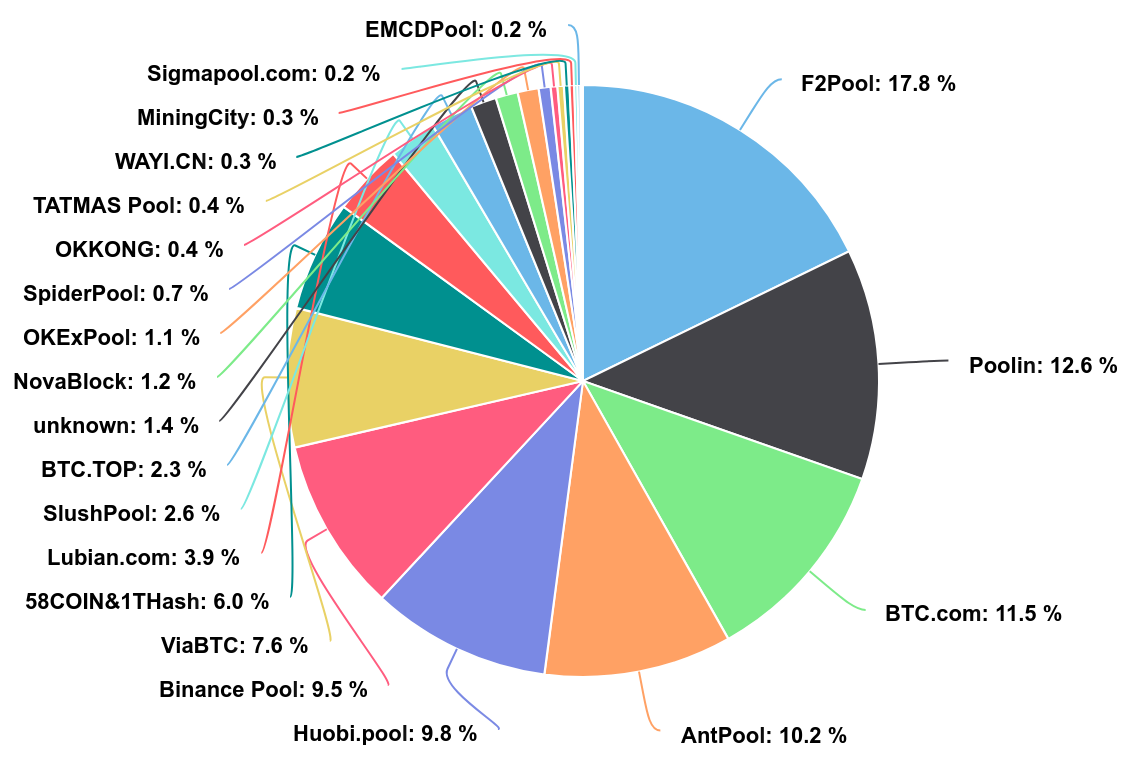
\includegraphics[width=0.75\linewidth]{pools.png}
    \caption{Rozdělení výpočetního výkonu bitcoinové sítě v~prosinci 2020~\cite{bib_pool_dist}.}
    \label{fig_pool_distribution}
\end{figure}

Formulace modelu, kdy těžař maximalizuje pouze počet utržených bitcoinů se zdá příliš zjednodušující. Těžaři své náklady (pořízení hardwaru, elektřina) pravděpodobně hradí v~dolarech (či jiné státní měně). Musí tedy bitcoiny prodat, z~toho zaplatit náklady a zbytek je jeho utržený zisk. Pokud by těžař uplatňoval strategii sobeckého těžení, tak sice za jistých podmínek utrží více bitcoinu, nicméně jeho celkový zisk se nezvýší, jelikož by bitcoin tratil na ceně. Těžař by spíše maximalizoval počet utržených bitcoinů $\times$ cena jednoho bitcoinu (např. v~amerických dolarech). Strategií sobeckého těžení by sice jednu složku tohoto výrazu zvýšil, ale druhou velmi pravděpodobně snížil.

Naopak se ukazuje, že v~zájmu těžařů je v~první řadě aby síť fungovala a lidé v~ní měli důvěru. V~roce 2014 pool Ghash.io pravděpodobně přesáhl hranici 50\% výpočetního výkonu sítě. Mohl tak teoreticky ignorovat práci všech ostatních, všechny bloky vytěžit sám a získat výrazně vyšší odměnu. Nic takového ale nenastalo. Samotný pool vydal prohlášení, že v~žádném případě nemá v~úmyslu Bitcoinu ublížit a že v~budoucnu už nepřesáhne 40\,\%. Těžaři poolu začali dobrovolně přecházet do jiných poolů~\cite{bib_coindesk_ghash}. V~současnosti žádný pool nepřesahuje těžební výkon 20\,\% (viz obrázek~\ref{fig_pool_distribution}).

%%%%%%%%%%%%%%%%%%%%%%%%%%%%%%%%%%%%%%%%%%%%%%%%%%%%%%%%%%%%%%%%%%%%%%%%%%%%%%%%
